\section{The p-adic group of type \texorpdfstring{$F_4$}{PDFstring}}

In this section, we verify Conjecture \ref{conj:main} for the split, simply connected $p$-adic group $G=F_4(F)$. Since the fundamental group $\Omega$ is trivial, $G$ is also adjoint. This is an important property that simple groups of type $F_4$ share with simple groups of type $G_2$ that simplify many calculations. Its dual group is $G^\vee=F_4(\CC)$, and we let $\{\alpha_1,\alpha_2,\alpha_3,\alpha_4\}$ be the simple roots of $G^\vee$, with Dynkin diagram 

\begin{center}
    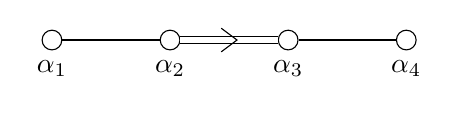
\begin{tikzpicture}[scale=1, baseline=-3pt, circ/.style={draw, circle, inner sep=2pt, minimum size=2.5mm}]
        \node[circ, label=below:$\alpha_1$] (1) at (0,0) {}; 
        \node[circ, label=below:$\alpha_2$] (2) at (1.5,0) {}; 
        \node[circ, label=below:$\alpha_3$] (3) at (3,0) {}; 
        \node[circ, label=below:$\alpha_4$] (4) at (4.5,0) {};
        \draw (1)--(2) (3)--(4);
        \draw[dashed] (2)--(3);
        \draw[double, double distance=2pt] (2) -- (3);
        \draw (2.15,0.15) -- (2.35,0) -- (2.15,-0.15);% Arrow
    \end{tikzpicture}
\end{center}
We denote by $\alpha_0$ and $\alpha^0$ the highest short root and highest long root of the root system, respectively, so the simple affine roots of $G$ are $S_{\aff}=\{-\calpha_0,\calpha_4,\calpha_3,\calpha_2,\calpha_1\}$ with affine Dynkin diagram 
\begin{center}
    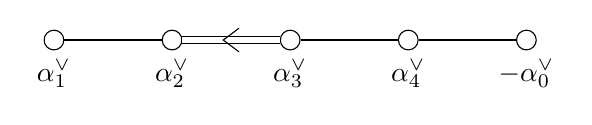
\begin{tikzpicture}[
        circ/.style={draw, circle, inner sep=2pt, minimum size=2.5mm}
    ]
        \node[circ, label=below:$\alpha^\vee_1$] (1) at (0,0) {};
        \node[circ, label=below:$\alpha^\vee_2$] (2) at (1.5,0) {};
        \node[circ, label=below:$\alpha^\vee_3$] (3) at (3,0) {};
        \node[circ, label=below:$\alpha^\vee_4$] (4) at (4.5,0) {};
        \node[circ, label=below:$-\alpha^\vee_0$] (0) at (6,0) {};

        \draw (1) -- (2);
        \draw[double, double distance=2pt] (3) -- (2);
        \draw (3) -- (4);
        \draw (4) -- (0);
        \draw (2.35,0.15) -- (2.15,0) -- (2.35,-0.15);% Arrow
    \end{tikzpicture}
\end{center}

The group $G$ has five maximal open compact subgroups $\{K_0,K_4,K_3,K_2,K_1\}$ up to conjugacy, where $K_i$ corresponds to $J_i:=S_{\aff}\setminus\{\alpha^\vee_i\}$ for $0\leq i\leq 4$. The reductive quotients $\overline{K}_0,\overline{K}_4,\overline{K}_3,\overline{K}_2$ and $\overline{K}_1$ are finite reductive groups of type $F_4, A_1\times C_3, A_2\times\tilde{A}_2, A_3\times\tilde{A}_1$ and $B_4$, respectively. In this section, we prove the following.

\begin{theorem}\label{thm:F4}
    Let $G$ be a simple p-adic group of type $F_4$. Then the diagram 
    \[
        \begin{tikzcd}
            R_{\un,\mathrm{ell}}(G) \arrow[r, "\FT^\vee_{\mathrm{ell}}"] \arrow[d, "\res_{\un}^{\mathrm{cpt}}"] & R_{\un,\mathrm{ell}}(G) \arrow[d, "\res_{\un}^{\mathrm{cpt}}"] \\
            \bigoplus_{i=0}^5 R_{\un}(\overline{K}_i) \arrow[r, "(\FT^{K_i})_i"] & \bigoplus_{i=0}^5 R_{\un}(\overline{K}_i),
        \end{tikzcd}
    \]
    commutes.
\end{theorem}

We remark that the above result was already proven by Ciubotaru, in an unpublished paper \cite{Ciubotaru2020} for the reduction to the hyperspecial parahoric subgroup $K_0$. We complete the proof for the remaining $4$ parahoric subgroups.

Firstly, we compute the basis $\{\Pi(u,s,h)\ |\ u\in G^\vee\text{ unipotent, } (s,h)\in\Gamma_u\backslash\mathcal{Y}(\Gamma_u)_{\mathrm{ell}}\}$ of the space $R_{\un,\text{ell}}(G)$ (see Section \ref{subsec:Fourier_transform} for the definitions). The classification of all elliptic pairs of $F_4(\CC)$ has been previously computed in the literature, and the list is given in Table \ref{tbl:F4_pairs}. For each unipotent $u\in F_4(\CC)$, we also give the unipotent $F_4(\FF_q)$-family $\mathcal{F}_u$ whose special element is the $W$-representation afforded by $\varepsilon\otimes H^{\mathrm{top}}(\mathcal{B}^u)^{\mathbf{1}}$ under the Springer correspondence. Then $\Gamma_{\mathcal{F}_u}$ is the finite group canonically associated to the family $\mathcal{F}_u$.

\begin{table}[ht]
    \centering
    \begin{tabular}{|c|c|c|c|c|c|}
        \hline
        Unipotent & $\Gamma_u^0$ & $A_u$ & $|\Gamma_u\backslash\mathcal(\Gamma_u)_{\text{ell}}|$ & $\mathcal{F}_{u}$ & $\Gamma_{\mathcal{F}_u}$ \\\hline
        $F_4$ & $1$ & $1$ & $1$ & $\phi_{1,24}$ & $1$ \\\hline
        $F_4(a_1)$ & $1$ & $S_2$ & $4$ & $\phi_{4,13}$ & $C_2$ \\\hline
        $F_4(a_2)$ & $1$ & $S_2$ & $4$ & $\phi_{9,10}$ & $1$ \\\hline
        $B_3$ & $\text{PGL}(2)$ & $1$ & $1$ & $\phi_{8,9}''$ & $1$ \\\hline
        $F_4(a_3)$ & $1$ & $S_4$ & $21$ & $\phi_{12,4}$ & $S_4$\\\hline
    \end{tabular}
    \caption{Elliptic pairs for $F_4$}
    \label{tbl:F4_pairs}
\end{table}

In particular, $E_{\un,\text{ell}}(G)$ is a $31$-dimensional vector space, where $21$ of these dimensions come from the distinguished unipotent class $F_4(a_3)$. The proof of Theorem \ref{thm:F4} relies on an explicit computation of the restriction map 
$$\res^{\mathrm{par}}_{\un}:\mathcal{R}_{\un,\mathrm{ell}}^p(G)\longrightarrow\bigoplus_{i=0}^5 R_{\un}(\overline{K}_i).$$
Most of this work was completed by Reeder in \cite{Reeder2000}. Nevertheless, his tables contain a few mistakes (systematically arising from the two representations $\pi(F_4(a_3),1,31)$ and $\pi(F_4(a_3),1,211)$) and do not include the representations whose unipotent label $u$ has type $B_3$ (for this is not a distinguished unipotent element of $F_4(\CC)$). We tabulate these results at the end of the section, fixing the mistakes and adding the new restrictions.

\iffalse To display this information for all unipotent classes simultaneously, we use the notation for the Langlands parameters as in \cite{Reeder2000}, which we now explain for convenience. 

\textbf{Notation:} Given a representation $\pi(x,\phi)$, let $x=us$ be the Jordan decomposition. Then $u\in Z_{G^\vee}(s)^0$ is a unipotent element of the connected pseudo-Levi subgroup $Z_{G^\vee}(s)^0$, and $\phi$ is an irreducible representation of the component group $A_{su}$. The representation $\pi(x,\phi)$ will be labelled by the type of unipotent element $u$ is inside $Z_{G^\vee}(s)^0$, together with the representation $\phi$. For example, if $u$ has type $F_4(a_3)$ and $s$ is a two-cycle, then $Z_{G^\vee}(s)$ has type $C_3\times A_1$, $u$ is labelled by $C_3(42)\times A_1$ (subregular in the first group and regular in the second) and $\widehat{A_{su}}=C_2\times C_2$. Thus, each representation has a name of the form $[u\in Z_{G^\vee}(s)^0,\phi]$ where $\phi$ is an irreducible representation of $A_{su}$.\fi

Let us briefly discuss how the parahoric restrictions are computed. The unipotent representations of $F_4(F)$ fall into $9$ unipotent blocks, together with their associated Hecke algebras. There are $7$ supercuspidal blocks, one for each cuspidal unipotent representation of $F_4(\FF_q)$. The corresponding Hecke algebras $\cH(F_4(F),F_4(\mathcal{O}_F),\sigma)$ are all isomorphic to $\CC$ so these blocks contain a unique unipotent representation. This information can be read from Lusztig's arithmetic-geometric correspondence tables in \cite{Lusztig1995}*{pg. 577}. The Langlands parameters of these representations are $$[F_4(a_3),1^4],\ [C_3(42),--],\ [B_4(531),\varepsilon],\ [2A_2,\theta],\ [2A_2,\theta^2],\ [A_1A_3,i]\text{ and }[A_1A_3,-i],$$
where we are using Notation \ref{notation:Langlandsparam} for the Langlands parameters. The parahoric restrictions of these representations are straightforward to compute, for they are irreducible for the hyperspecial parahoric $K_0$ and vanish for the other ones.

The principal block contains all Iwahori-spherical representations, that is, all representations $\pi(us,\phi)$ such that $H(\mathcal{B}_s^u)^{\phi}\neq 0$. The corresponding Hecke algebra $\cH(F_4(F),I,\mathbf{1})$ is the affine Hecke algebra of type $F_4$ with equal parameters. We compute the parahoric restrictions, using Springer theory, the Green tables of $F_4(\FF_q)$ and the methods described in subsection \ref{subsec:Iwahori_spherical}.

%The parahoric restrictions to the maximal hyperspecial $K_0$ are computed using Springer theory and the Green functions of $F_4(\FF_q)$, which are explicitly known thanks to the work of Beynon-Spaltenstein in \textcolor{red}{Cite BeynonSpaltenstein1984}. The results are tabulated at the end of the section. To compute the parahoric restrictions to the other maximal parahoric subgroups, we use \eqref{eqn:mackey_generalcase}, which relies on the computation of the groups $W_{J,t}$ and the characters $\chi_t^J$. In many instances, the characters are trivial (for example, if $W_{J,t}$ is a reflection subgroup of $W_J$); when this is the case, we use Lemma \ref{lem:mackey_restriction}. The restriction can then be easily obtained from Alvis' tables \textcolor{red}{Insert the reference here}.

Finally, there is an intermediate block whose Hecke algebra $\cH(F_4(F),B_2,\sigma)$ is the affine Hecke algebra of type $C_2$ with unequal parameters that we introduced in Example \ref{ex:F4_B2_algebra}. All Langlands parameters of the representations of interest in this block are \textit{elliptic}, so it suffices to compute the square integrable representations of $\cH(F_4(F),B_2,\sigma)$ to determine the desired parahoric restrictions. This can be achieved using the theory of weight diagrams briefly discussed in Section \ref{sec:weight_diagram} (see also \cite{Ciubotaru2020}*{\S 9}). The Langlands parameters of these representations are $$[B_4,-],\ [C_3A_1,-],\ [C_3(42)A_1,-+],\ [B_4(531),r] \text{ and } [A_1A_3,-1].$$ 
We explicitly discuss the $[A_1A_3,-1]$ case in Example \ref{ex:A1A3}, and we tabulate the rest of the parahoric restrictions at the end of the section.

Before displaying the tables, let us discuss a few examples in detail to illustrate the main ideas involved in the calculations. We will focus on the representations whose unipotent part has type $F_4(a_3)$, since they are the most interesting. 

\subsection{Examples of parahoric restrictions}
The first example is the computation of a parahoric restrictions with respect to the maximal hyperspecial parahoric $K_0$ using Springer Theory and Alvis' tables.

\begin{example}
    Consider the representation $[B_4(531),\mathbf{1}]$, with $u$ of type $F_4(a_3)$ and $s\in\Gamma_u$ a product of two $2$-cycles. The centralizer $Z_{G^\vee}(s)$ has type $B_4$ and $u\in Z_{G^\vee}(s)$ is subregular. Thus, the Springer fibre $\cB^u_s$ is $2$ dimensional, and by reading the Green functions we obtain
    $$H^*(\cB^u_s)^\mathbf{1}=[2,2]+[3,1]+[4,\cdot]\quad\text{as $W_s$-modules}.$$
    Since all characters are trivial when $J=J_0$, Alvis' tables yield
    $$\Ind_{W_s}^W[2,2]+[3,1]+[4,\cdot]=\phi_{9,2}+\phi_{9,6}''+\phi_{8,3}''+\phi_{4,1}+\phi_{2,4}''+\phi_{1,0}.$$
    To obtain the parahoric restriction of the representation $[B_4(531),\mathbf{1}]$ with respect to $K_0$, we twist by $\varepsilon$ and by the outer automorphism of $W$ swapping long and short roots, so
    $$[B_4(531),\mathbf{1}]\xrightarrow{\res^{K_0}_{\un}}\phi_{9,10}+\phi_{9,6}''+\phi_{8,9}''+\phi_{4,13}+\phi_{2,16}''+\phi_{1,24}.$$
\end{example}
Once the parahoric restrictions for the maximal hyperspecial have been calculated, we can turn our attention towards computing the rest. The first step is to determine when the characters $\chi_t^J$ are trivial. The order of the semisimple elements $s$ in the Langlands parameters are clear, while one can show that $Z_{J_1},Z_{J_2},Z_{J_3}$ and $Z_{J_4}$ have order $2,2,3$ and $2$, respectively. Whenever the orders of $s$ and $J_1$ are relatively prime the characters are trivial, and we can use Lemma \ref{lem:mackey_restriction} and Alvis' tables to compute the restriction directly. Let us discuss another interesting example.

\begin{example}
    Consider the parahoric restriction of the Iwahori-spherical representation $[A_1A_3,\mathbf{1}]$, where $u$ is of type $F_4(a_3)$ and $s\in\Gamma_u$ is a $4$-cycle, with respect to the parahoric subgroup $K_2$. Note that $W_{J_2}=\langle s_0,s_4,s_3,s_1\rangle\cong W(A_3)\times W(A_1)$. The semisimple part $s$ can be chosen to be $s=\calpha_3(-1)\calpha_4(i)$ so that $W_s=\langle s_4,s_2,s_1,s^0\rangle\cong W(A_1)\times W(A_3)$. In addition, $u$ is a regular unipotent element in $Z_{G^\vee}(s)$, so $H^*(\mathcal{B}_s^u)^{\mathbf{1}}=\mathbf{1}$ as a $W_s$-module. Next,
    $$W_s\backslash W/W_{J_2}=\{1,w\},$$
    where $w\in W$ is explicitly computable with computer algebra programs such as GAP. In addition, 
    $$W_{J_2,s}=\langle s_4,s_1\rangle\cong C_2\times C_2,\quad\text{while}\quad W_{J_2,s^w}=\langle d \rangle\cong C_4,$$
    for some $d\in W$ of order $4$. Since $W_{J_2,s}$ is a reflection subgroup of $W_{J_2}$, the character $\chi_s^{J_2}$ is trivial. On the other hand, $W_{J_2,s^w}$ is not a reflection subgroup of $W_{J_2}$, and $\chi_{s^w}^{J_2}=\chi$ is a primitive character of $C_4$. The induced representations are then given by
    \begin{align*}
        \Ind_{W_{J_2,s}}^{W_{J_2}}\mathbf{1}=[[4]+2[311]+[22]+[211]]\boxtimes[2]\quad\text{and}\quad\Ind_{W_{J_2,s^w}}^{W_{J_2}}\chi=[[31]+[211]]\boxtimes[[2]+[11]].
    \end{align*}    
    Adding these and twisting by sign gives the required parahoric restriction.
\end{example}



\begin{example}
    A more challenging example is the calculation of the parahoric restriction of $[2A_2,\mathbf{1}]$, with $u$ of type $F_4(a_3)$ and $s\in\Gamma_u$ is a $3$-cycle, with respect to $K_3$. This is the only case where a characters $\chi_{s^w}^{J_3}$ may be non-trivial. Note that $W_{J_3}=\langle s_0,s_4,s_2,s_1\rangle\cong W(A_2)\times W(A_2)$.
    The semisimple part can be taken to be $s=\calpha_3(\xi_3)\calpha_4(\xi_3^2)$, where $\xi_3$ is a primitive third root of unity. In particular, $Z_{G^\vee}(s)$ is a pseudo-Levi subgroup of type $A_2\times A_2$ generated by the affine simple roots $\{\alpha_4,\alpha_3,\alpha_1,-\alpha^0\}$ and $W_s=\langle s_4,s_3,s_1,s^0\rangle$. In addition, the unipotent element $u$ is regular in $Z_{G^\vee}(s)$, so $H^*(\cB^u_s)^{\mathbf{1}}=\mathbf{1}$ as $W_s$-modules. Next,
    $$W_s\backslash W/W_{J_3}=\{w_1=1,w_2,w_3,w_4,w_5\},$$
    where $w_i\in W$ are representatives of double cosets with sizes $324, 324, 36, 36$ and $432$, respectively. The subgroups 
    $$W_{J_3,s^{w_3}}=W_{J_3,s^{w_4}}=W_{J_3}\quad\text{and}\quad W_{J_3,s}\cong W_{J_3,s^{w_2}}\cong C_2\times C_2$$
    are all reflections subgroups of $W_{J_3}$, so the characters $\chi_{s^{w_i}}^{J_3}$ are trivial for $i=1,2,3,4$. The remaining coset is more interesting since    
    $$W_{J_3,s^{w_5}}=\langle d \rangle\cong C_3,$$
    is no longer a reflection subgroup, and $\chi_{s^{w_4}}^{J_3}$ is a primitive character $\chi$ of $C_3$. 
    
    The induced representations are then given by
    \begin{align*}
        \Ind_{W_{J_3,s}}^{J_3}\mathbf{1}=\Ind_{W_{J_3,s^{w_2}}}^{J_3}\mathbf{1}=&[3,3]+[3,21]+[21,3]+[21,21],\quad\Ind_{W_{J_3,s^{w_3}}}^{J_3}\mathbf{1}=\Ind_{W_{J_3,s^{w_4}}}^{J_3}\mathbf{1}=[3,3]\\
        \text{and}\quad&\Ind_{W_{J_3,s^{w_5}}}^{J_3}\chi=[21,3]+[3,21]+[21,21]+[21,1^3]+[1^3,21].
    \end{align*}
    Adding these and twisting by sign gives the required parahoric restriction.
\end{example}

Finally, let us discuss the parahoric restrictions of the non-Iwahori-spherical representation $[A_1A_3,-1]$.

\begin{example}\label{ex:A1A3}
    Let $V$ be the representation labelled by $[A_1A_3,-1]$, $K$ a parahoric subgroup of type $B_2$ and let $\sigma$ be the unique cuspidal unipotent representation of $B_2(\FF_q)$. Since the types of the reductive quotients of $K_2$ and $K_3$ ($A_3\times\tilde{A}_1$ and $A_2\times\tilde{A}_2$, respectively) do not contain $B_2$ as a factor, the parahoric restrictions of $V$ to $K_2$ and $K_3$ vanish. 

    On the other hand, $V^\sigma$ is a square integrable representation of $\cH(F_4(F),B_2,\sigma)\cong\cH(K_{J_0},K,\sigma)\tilde\otimes\mathcal{O}[\mathbf{T}]$, whose restriction to $\mathcal{O}[\mathbf{T}]$ is
    $$V^\sigma|_{\mathcal{O}[\mathbf{T}]}=V^\sigma(q^{-2},-q^{-1})\oplus V^\sigma(-q^{-1},q^{-2}),$$
    both subspaces being one-dimensional. By choosing a basis element in each subspace, the rational functions $e_{\alpha_1}, e_{\alpha_2}\in\mathcal{O}[\mathbf{T}]$ act on $V^\sigma$ by $\mathrm{diag}(-q^{-1},-q)$ and $\mathrm{diag}(-q^{-1},q^{-2})$. Using the formula for the twisted multiplication in $\cH(F_4(F),B_2,\sigma)$, the action of the generators $T_1$ and $T_2$ can be computed explicitly, and we obtain
    \begin{equation*}
        T_{s_1}\longrightarrow\frac{1}{q+1}\begin{pmatrix}
            q^3-1 & q^3+q \\
            q^4+1 & q^4-q
        \end{pmatrix}\quad\text{and}\quad T_{s_2}\longrightarrow\begin{pmatrix}
            -1 & 0 \\
            0 & -1
        \end{pmatrix}.
    \end{equation*}
    Finally, one can trace back through the isomorphisms $\cH(F_4(F),B_2,\sigma)\cong\cH(K_{J_0},K,\sigma)\ \tilde\otimes\ \mathcal{O}[\mathbf{T}]$ to obtain that $T_{\tilde{s}_0}$ acts by
    \begin{equation*}
        T_{\tilde{s}_0}\longrightarrow\frac{1}{q^3+q^2}\begin{pmatrix}
            -q^6+q^3-q^2-1 & q^5+q^3-q^2-1 \\
            -q^7+q^4-q^3+1 & q^6+q^4-q^3+1
        \end{pmatrix}.
    \end{equation*}
    Thus, the action of $\tilde{W}(K,\sigma)$ on $V^\sigma_{q=1}$ is given by
    \begin{equation*}
        s_1\longrightarrow\begin{pmatrix}
            0 & 1 \\
            1 & 0
        \end{pmatrix},\quad s_2\longrightarrow\begin{pmatrix}
            -1 & 0 \\
            0 & -1
        \end{pmatrix}\quad\text{and}\quad \tilde{s}_0\longrightarrow\begin{pmatrix}
            -1 & 0 \\
            0 & 1
        \end{pmatrix}.
    \end{equation*}
    The parahoric restrictions are now obtained by restricting to reflection subgroups. Restriction to the reflection subgroup $\langle s_1,s_2\rangle\cong W(B_2)$ gives the parahoric restriction to $K_0$, restriction to $\langle s_1,\tilde{s}_0\rangle\cong W(B_2)$ gives the parahoric restriction to $K_1$ and restriction to $\langle s_2,\tilde{s}_0\rangle\cong W(A_1\times A_1)$ gives the parahoric restriction to $K_4$. In each case, there is a bijection between representations of the Weyl group and unipotent representations of $\overline{K}_i$ in the series generated by $\sigma$, which we use implicitly. Throughout, we use Lusztig's notation for the unipotent representations. We obtain
    \begin{itemize}
        \item Firstly, $V^\sigma|_{\langle s_1,s_2\rangle}=[11,\emptyset]+[\emptyset,11]$, so $[A_1A_3,-1]\xrightarrow{\res^{K_0}_{\un}}B_2[\varepsilon']+B_2[\varepsilon].$
        \item Secondly, $V^\sigma|_{\langle s_1,\tilde{s}_0\rangle}=[1,1]$, so $[A_1A_3,-1]\xrightarrow{\res^{K_1}_{\un}}\begin{psmallmatrix}
            0 \ 1\ 2\ 4\\
            \ \ \ 1 \ \ \
        \end{psmallmatrix}$.
        \item Finally, $V^\sigma|_{\langle s_2,\tilde{s}_0\rangle}=[11]\boxtimes[2]+[11]\boxtimes[11]$, so $[A_1A_3,-1]\xrightarrow{\res^{K_4}_{\un}}\begin{psmallmatrix}
            0 \ 1\ 2\ 3\\
            \ \ \ 1 \ \ \
        \end{psmallmatrix}\boxtimes\mathbf{1}+\begin{psmallmatrix}
            0 \ 1\ 2\ 3\\
            \ \ \ 1 \ \ \
        \end{psmallmatrix}\boxtimes\St.$
    \end{itemize}
\end{example}


\iffalse

For the purposes of this document, we will instead just discuss in detail a few examples that already highlight the main ideas involved in the calculation for distinct parahoric subgroups $K_i$. All examples discussed come from Iwahori-spherical representations, since the parahoric restrictions of the other representations are still work in progress. This work was mostly completed by \cite[\S 10]{Reeder2000}, but his tables contain some mistakes, systematically arising from the two representations $\pi(F_4(a_3),1,31)$ and $\pi(F_4(a_3),1,211)$. We have been unable to guess where the mistake may have come from. We gather all the results in large tables at the end of the section that fix the mistakes in Reeder's tables. We omit the tables for the parahoric restriction to maximal hyperspecial for a few reasons; they take the most space, the are already correct in Reeder's paper (except for the restriction of $[B_4(531),\epsilon'']$, where the second $K_0$ type should be $\phi_{2,16}'$ instead of $\phi_{2,16}''$) and Theorem \ref{thm:F4} has already been proven in this case.

The conjecture can be verified one unipotent class $u\in G^\vee$ at a time. By far, the most interesting case is the class $F_4(a_3)$, so all examples will involve representations labelled by this class. Let us introduce some helpful notation used in \cite{Reeder2000}. The class $F_4(a_3)$ is distinguished with component group isomorphic to $S_4$, so there are $5$ conjugacy classes of semisimple elements commuting with any $u\in F_4(a_3)$. If $s$ is such a semisimple element, then $Z_{G^\vee}(s)$ is a pseudo-Levi subgroup of a certain type, and $u$ is a unipotent element of this group with a certain label. Then the representation of $F_4(F)$ parametrized by $(us,\phi),\phi\in\widehat{A_{su}}$ will be labelled by the type of unipotent $u$ inside $Z_{G^\vee}(s)$, together with the representation $\phi$.

For example, if $s$ is a two-cycle, then $Z_{G^\vee}(s)$ has type $C_3\times A_1$, $\widehat{A_{su}}=C_2\times C_2$ and $u$ is labelled by $C_3(42)\times A_1$ (subregular in the first group and regular in the second). If $s$ is a three-cycle, then $Z_{G^\vee}(s)$ has type $A_2\times A_2$, $\widehat{A_{su}}$ and $u$ is a regular unipotent labelled by $2A_2$. See the tables at the end for all the labels.

\fi